\documentclass[11pt,fleqn]{book}
\usepackage[letterpaper]{geometry}
\usepackage{graphicx}    % needed for including graphics e.g. EPS, PS
\usepackage{amsmath}
\usepackage{xfrac}
\usepackage[version=4]{mhchem}
\usepackage{listings}
\usepackage{hyperref}
\usepackage{wrapfig}
\usepackage{empheq}
\usepackage{capt-of}
\usepackage{tcolorbox}

%\usepackage[print]{booklet}

% To use UTF-8 characters
\usepackage[utf8x]{inputenc}
% \DeclareUnicodeCharacter{207A}{$^+$}
% \DeclareUnicodeCharacter{207B}{$^-$}







% color def PYTHON CODE
\usepackage{color}
\definecolor{darkred}{rgb}{0.6,0.0,0.0}
\definecolor{darkgreen}{rgb}{0,0.50,0}
\definecolor{lightblue}{rgb}{0.0,0.42,0.91}
\definecolor{orange}{rgb}{0.99,0.48,0.13}
\definecolor{grass}{rgb}{0.18,0.80,0.18}
\definecolor{pink}{rgb}{0.97,0.15,0.45}

% listings
\usepackage{listings}

% General Setting of listings
\lstset{
	aboveskip=1em,
	breaklines=true,
	abovecaptionskip=-6pt,
	captionpos=b,
	escapeinside={\%*}{*)},
	frame=single,
	numbers=left,
	numbersep=15pt,
	numberstyle=\tiny,
}
% 0. Basic Color Theme
\lstdefinestyle{colored}{ %
	basicstyle=\ttfamily,
	backgroundcolor=\color{white},
	commentstyle=\color{green}\itshape,
	keywordstyle=\color{blue}\bfseries\itshape,
	stringstyle=\color{red},
}
% 1. General Python Keywords List
\lstdefinelanguage{PythonPlus}[]{Python}{
	morekeywords=[1]{,as,assert,nonlocal,with,yield,self,True,False,None,} % Python builtin
	morekeywords=[2]{,__init__,__add__,__mul__,__div__,__sub__,__call__,__getitem__,__setitem__,__eq__,__ne__,__nonzero__,__rmul__,__radd__,__repr__,__str__,__get__,__truediv__,__pow__,__name__,__future__,__all__,}, % magic methods
	morekeywords=[3]{,object,type,isinstance,copy,deepcopy,zip,enumerate,reversed,list,set,len,dict,tuple,range,xrange,append,execfile,real,imag,reduce,str,repr,}, % common functions
	morekeywords=[4]{,Exception,NameError,IndexError,SyntaxError,TypeError,ValueError,OverflowError,ZeroDivisionError,}, % errors
	morekeywords=[5]{,ode,fsolve,sqrt,exp,sin,cos,arctan,arctan2,arccos,pi, array,norm,solve,dot,arange,isscalar,max,sum,flatten,shape,reshape,find,any,all,abs,plot,linspace,legend,quad,polyval,polyfit,hstack,concatenate,vstack,column_stack,empty,zeros,ones,rand,vander,grid,pcolor,eig,eigs,eigvals,svd,qr,tan,det,logspace,roll,min,mean,cumsum,cumprod,diff,vectorize,lstsq,cla,eye,xlabel,ylabel,squeeze,}, % numpy / math
}
% 2. New Language based on Python
\lstdefinelanguage{PyBrIM}[]{PythonPlus}{
	emph={d,E,a,Fc28,Fy,Fu,D,des,supplier,Material,Rectangle,PyElmt},
}
% 3. Extended theme
\lstdefinestyle{colorEX}{
	basicstyle=\ttfamily,
	backgroundcolor=\color{white},
	commentstyle=\color{darkgreen}\slshape,
	keywordstyle=\color{blue}\bfseries\itshape,
	keywordstyle=[2]\color{blue}\bfseries,
	keywordstyle=[3]\color{grass},
	keywordstyle=[4]\color{red},
	keywordstyle=[5]\color{orange},
	stringstyle=\color{darkred},
	emphstyle=\color{pink}\underbar,
}









\usepackage{tikz}
\usepackage{tikzpagenodes}
\usetikzlibrary{positioning}

\topmargin -1.5cm        % read Lamport p.163
\oddsidemargin -0.04cm   % read Lamport p.163
\evensidemargin -0.04cm  % same as oddsidemargin but for left-hand pages
%\textwidth 16.59cm
\textwidth 11cm
\textheight 21.94cm 
%\pagestyle{empty}       % Uncomment if don't want page numbers
\parskip 7.2pt           % sets spacing between paragraphs
%\renewcommand{\baselinestretch}{1.5} 	% Uncomment for 1.5 spacing between lines
\parindent 0pt		  % sets leading space for paragraphs


\newcounter{qNum}
\newcommand{\qn}{\refstepcounter{qNum} \theqNum}
\newcounter{qNumH}
\newcommand{\qnH}{\refstepcounter{qNumH}  \textit{Honors} \theqNumH}
\newcommand{\eqn}{\text{\qn) \ }}
\def \dt {\ensuremath{\,\mathrm{d}t}}

\newcommand{\aspace}{ \hspace{1em}\\ \vspace{8em}}

\newcommand{\dx}{\; dx}

\newcommand{\D}[1]{\; d{#1}}

\newcommand{\graphGrid}{
	
\begin{tikzpicture}
	\draw[step=.5cm,gray,help lines] (-5,-5) grid (5,5);
	\draw[step=2.5cm,black,very thin] (-5,-5) grid (5,5);
	\end{tikzpicture}
}

\newcommand{\graphGridAxes}{
	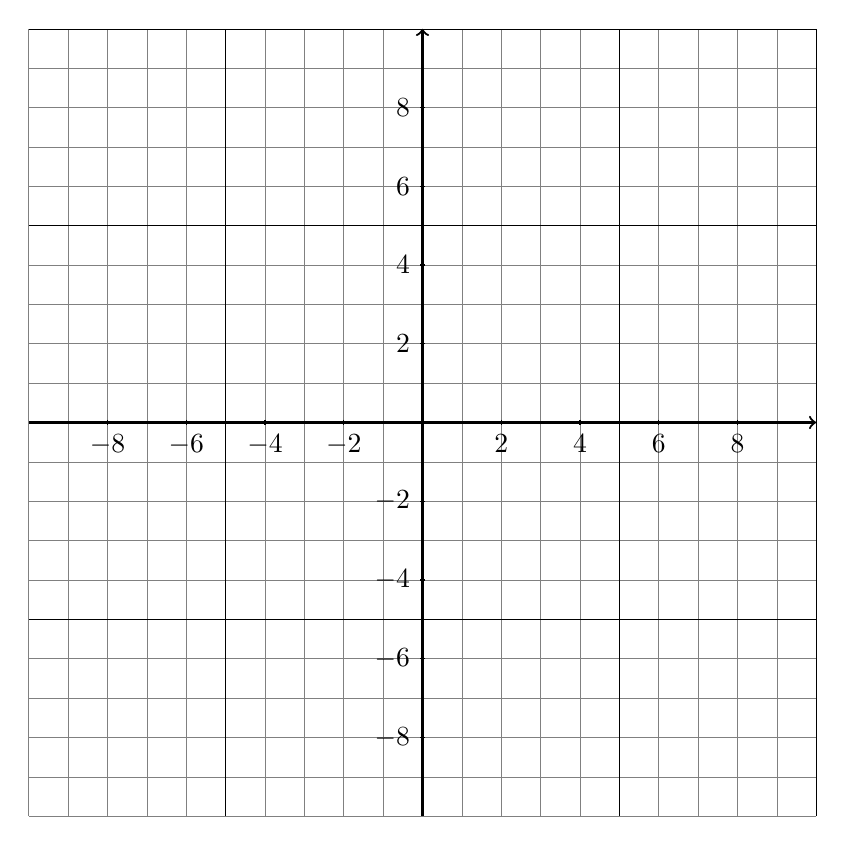
\begin{tikzpicture}
	\draw[step=.5cm,gray,help lines] (-5,-5) grid (5,5);
	\draw[step=2.5cm,black,very thin] (-5,-5) grid (5,5);
	\draw[thick,->] (-5,0) -- (5,0) ;
	\draw[thick,->] (0,-5) -- (0,5) ; 
	\foreach \x in {-8, -6, -4, -2,  2,4, 6, 8}
	\draw (\x*0.5 cm,1pt) -- (\x*0.5 cm,-1pt) node[anchor=north] {$\x$};
	\foreach \y in {-8, -6, -4, -2,  2,4, 6, 8}
	\draw (1pt,\y*0.5 cm) -- (-1pt,\y*0.5 cm) node[anchor=east] {$\y$};
	\end{tikzpicture}
}

\newcommand{\graphGridAxesS}[1]{
	\begin{tikzpicture}
		\draw[step=.5cm,gray,help lines] (-0.5*#1,-0.5*#1) grid (0.5*#1, 0.5*#1);
		\draw[step=2.5cm,black,very thin] (-0.5*#1,-0.5*#1) grid (0.5*#1, 0.5*#1);
		\draw[thick,->] (-#1/2,0) -- (#1/2,0) ;
		\draw[thick,->] (0,-#1/2) -- (0,#1/2) ; 
		\foreach \x in {-8, -6, -4, -2,  2,4, 6, 8}
		\draw (\x*0.5 cm,1pt) -- (\x*0.5 cm,-1pt) node[anchor=north] {$\x$};
		\foreach \y in {-8, -6, -4, -2,  2,4, 6, 8}
		\draw (1pt,\y*0.5 cm) -- (-1pt,\y*0.5 cm) node[anchor=east] {$\y$};
	\end{tikzpicture}
}



%headers
\usepackage{datetime}
\usepackage{fancyhdr}
\pagestyle{fancy}
\lhead{ }
\rhead{\footnotesize Finite Difference Method: Cylindrical Tube (\monthname, \the\year)}
\title{Introduction to the Finite Difference Method: \\ Filling and Draining a Cylindrical Tube}
\author{Lensyl Urbano}



 \begin{document}         
 % Start your text
 
\maketitle



\chapter{Filling a Cylindrical Tube}


Consider filling a cylinder with water. 


	\begin{tikzpicture}[remember picture,overlay,shift={(current page.east)}]
		\node[anchor=north east,xshift=-2cm](myImage){
			%\centering
			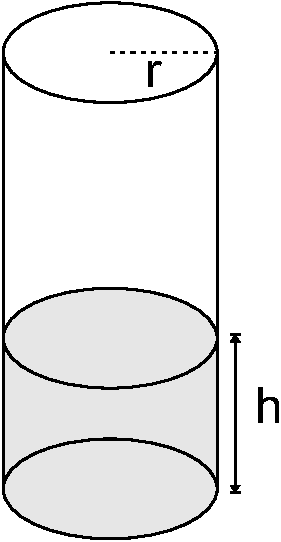
\includegraphics[height=5cm]{cylinder-rh.pdf} 
		};
		\node[inner sep=0pt,text width=0.5\linewidth] (myCaption) [below=of myImage]
	{\captionof{figure}{Cylinder with dimensions. $r$ is the radius and $h$ is the height of water in the tube.}};
	\end{tikzpicture}




The water flows in at a constant rate of 5 cm$^3$/s. The inflow rate ($Q$) can be written as the change in volume ($V$) over the change in time ($t$) (the $\Delta$ symbol represents change):

\textbf{Inflow Rate}
\begin{equation}
	Q = \frac{\Delta V}{\Delta t} = 5 \; cm^3/s
\end{equation}



\section{Filling the Tube Calculations and Equations}

\subsection{Conceptual Physics Approach}

		      
	So, at this inflow rate, after 10 seconds there will be 50 cm$^3$ added to the cylinder.
		\begin{align*}
			 V &= 5 \; cm^3/s \cdot 10 \; s \\
					&= 50 \; cm^3
		\end{align*}
	
	In terms of the equation, the change in volume is equal to the inflow rate ($Q$) times the time period ($ t$).
	  \begin{equation}
	  	\label{Vrate}
	  	 V = Q \cdot t \\
	  \end{equation}
	
	How high will the water have risen in the cylinder in those 10 seconds when 50 cm$^3$ of water was added? Well, we know that the volume of a cylinder is given by the equation:
		\begin{equation}
			V = \pi r^2 h
		\end{equation}
	
	So, if we know the volume and the radius of the cylinder ($r$) we can solve this equation for the height ($h$):
	
	Divide both sides by $\pi r^2$:
		\begin{equation}
			\frac{V}{\pi r^2} = \frac{\pi r^2 h}{\pi r^2}
		\end{equation}
	
	To get:
		\begin{equation}
			\frac{V}{\pi r^2} = h 
		\end{equation}
	
	Which can be rewritten as:
		\begin{equation}
			h = \frac{V}{\pi r^2}  
		\end{equation}
	
	or:
		\begin{equation}
			h = \frac{1}{\pi r^2} V
		\end{equation}
	
	Thus, for our given problem where the radius is 2.25 cm, and the volume of water added is 50 cm$^3$:
		\begin{equation}
			h = \frac{1}{\pi \cdot 2.25^2} \cdot 50 = 3.1 \; \text{cm}
		\end{equation}
	
	
	Now we can substitute for volume using Equation \ref{Vrate} to get:
		\begin{equation}
			h = \frac{1}{\pi r^2} \; Q \cdot t
		\end{equation}
	
	Now, lets rewrite this equation so we just consider what happens over a small time period (call it a \textit{time step} denoted by $\Delta t$). It's the change from moment to moment and results in a small change in height ($\Delta h$). So our final equation becomes:
		\begin{equation}
			\Delta h = \frac{1}{\pi r^2} \; Q \cdot \Delta t
		\end{equation}
	
	Which we rearrange a little to get:
		\begin{empheq}[box=\fbox]{equation}
			\label{dh_eqn}
			\Delta h = \frac{\Delta t}{\pi r^2} \; Q 
		\end{empheq}
	
	Having calculated the change in the height of the water in the cylinder in a given time step ($\Delta t$), for each timestep we calculate the new height of water ($h_{new}$) as the old height plus the change:
		\begin{empheq}[box=\fbox]{equation}
			\label{hnew_eqn}
			h_{new} = h_{old} + \Delta h
		\end{empheq}
	
	We can now use these two equation to create a computer model that gives the height of water in the column over time.
	

\subsection{Using Calculus to Find the Discrete Equations} \label{CodeCalc}

	Same problem--filling a cylinder--but using calculus to end up with the same equations in the end.
	
	Start with the equation for the volume of a cylinder:
		\begin{equation}
			V = \pi r^2 h
		\end{equation}
	
	There are two variables that change with time as the cylinder fills, the volume ($V$) and the height ($h$) since the radius ($r$) does not change. So, if we differentiate this equation with respect to time (implicit differentiation), we get:
		\begin{equation}
			\frac{dV}{dt} = \pi r^2 \frac{dh}{dt} 
		\end{equation}
	
	Solving for $\frac{dh}{dt}$ gives the \textbf{height change equation}:
		\begin{equation}
			\label{eqn:heightChange}
			\frac{dh}{dt} = \frac{1 }{\pi r^2 } \frac{dV}{dt}
		\end{equation}

	The expression $\frac{dh}{dt}$ represents the instantaneous change in height with time: the rate at which height changes at any instant. To write a program to solve this equation we'll \textbf{discretize} the expression by using $\frac{\Delta h}{\Delta t}$:
		\begin{equation}
			\frac{\Delta h}{\Delta t} \approx \frac{dh}{dt} 
		\end{equation}
		
	The $\Delta$ means that we're taking the difference between two discrete value of $h$, so:
		\begin{equation}
			\Delta h = h_2 - h_1
		\end{equation}
	
	Since this is the rate of change over time it can be easier to think of the change in height as the difference between the new height and the old height over the short ($\Delta t$) time period.
		\begin{equation}
			\label{eqn:discrete_h}
			\Delta h = h_{new} - h_{old}
		\end{equation}
	
	So now we rewrite our height change equation (Eqn. \ref{eqn:heightChange}) as:
		\begin{equation}
			\frac{\Delta h}{\Delta t} = \frac{1 }{\pi r^2 } \frac{dV}{dt}
		\end{equation}
		
	which we can solve for the change in height ($\Delta h$):
		\begin{equation}
		\Delta h = \frac{\Delta t }{\pi r^2 } \frac{dV}{dt}
		\end{equation}
	
	Since the inflow rate ($Q$) is the change in volume over time, and it remains constant for our model, we can say:
	
	\textbf{Change in Height Equation}
		\begin{empheq}[box=\fbox]{equation}
			\label{eqn:dh_calc}
			\Delta h = \frac{\Delta t }{\pi r^2 } \; Q
		\end{empheq}
	
	Which is the same equation (Eqn. \ref{dh_eqn}) we found when we took the conceptual approach in the previous section.
	
	Now we substitute in the discrete change for $\Delta h$ (Eqn. \ref{eqn:discrete_h}) to get:
		\begin{equation}
			 h_{new} - h_{old} = \frac{\Delta t }{\pi r^2 } \; Q
		\end{equation}
	
	Which we can solve for the new height:
		\begin{equation}
			h_{new} = h_{old} + \frac{\Delta t }{\pi r^2 } \; Q
		\end{equation}
	
	
	Which is the same as:
	
	\textbf{Height Update Equation}
		\begin{empheq}[box=\fbox]{equation}
			\label{eqn:dh_discrete}
			h_{new} = h_{old} + \Delta h 
		\end{empheq}
	
	We can use the \textbf{Change in Height} (Eqn. \ref{eqn:dh_calc}) and \textbf{Height Update} (Eqn. \ref{eqn:discrete_h}) equations to create a computer model of the height of the water in the cylinder as it fills it up.

\newpage
\section{Code}

	The following example code that solves this water-filling problem uses the \href{https://github.com/lurbano/ezGraph}{ezGraph class} \\ (https://github.com/lurbano/ezGraph) which requires matplotlib and numpy. However, the code in the following section avoids the use of most imported modules, but does not graph.
	
	\subsubsection{Code with Graphical Output}
	
		\textit{water-filling-fd.py}
		\begin{tikzpicture}[remember picture,overlay,shift={(current page.east)}]
			\node[anchor=north east,xshift=-1cm](fillingOutput){
				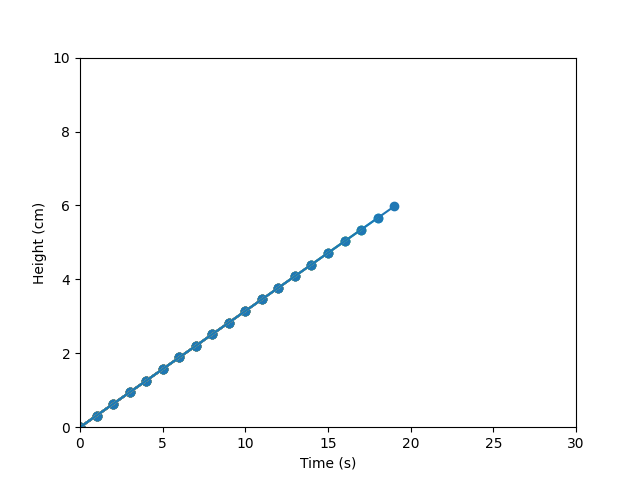
\includegraphics[height=5cm]{water-filling-fd.png} 
			};
			\node[inner sep=0pt,text width=0.5\linewidth] (myCaption) [below=of myImage]
			{\captionof{figure}{\label{fillingModel} Model output: Graph of height of water in the column over time when filling the cylinder.  }};
		\end{tikzpicture}
	
		\lstinputlisting[language=Python, frame=single]{../water-filling-fd.py}

	
	
%	\begin{figure}[h] 
%		\caption{Model output: Graph of height of water in the column over time when filling the cylinder.}
%		\centering
%		\label{fillingModel}
%		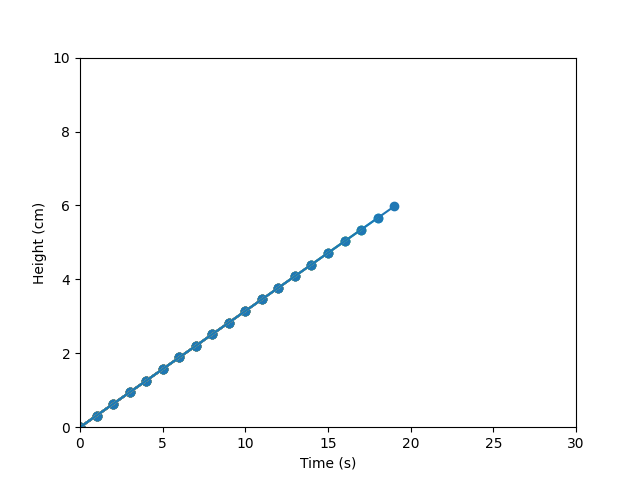
\includegraphics[width=0.75\textwidth]{water-filling-fd.png}
%	\end{figure}
	
	\subsection{Code without Graphical Output}
	A stripped down version of the code with no graph and no external modules except "math".
	
	\textit{water-filling-fd-noGraph.py}
	\lstinputlisting[language=Python, frame=single]{../water-filling-fd-noGraph.py}
	
	
	Which should produce a table of time and height output:
	
	\begin{lstlisting}
0 0
1.0 0.31438013450250935
2.0 0.6287602690050187
3.0 0.943140403507528
4.0 1.2575205380100374
5.0 1.5719006725125468
6.0 1.8862808070150563
7.0 2.2006609415175657
8.0 2.515041076020075
9.0 2.8294212105225847
10.0 3.143801345025094
11.0 3.4581814795276036
12.0 3.772561614030113
13.0 4.086941748532622
14.0 4.4013218830351315
15.0 4.715702017537641
16.0 5.03008215204015
17.0 5.34446228654266
18.0 5.658842421045169
19.0 5.973222555547679
	\end{lstlisting}



\section{Analytical Solutions using Calculus}

	The analytical solution to this problem will help confirm the accuracy of our model.+

	\subsection{Filling}

	As we saw in the section on using calculus (Section \ref{CodeCalc}), we can start with the equation for the volume of a cylinder:
	\begin{equation}
		V = \pi r^2 h
	\end{equation}
	
	And differentiate with respect to time to get:
	\begin{equation}
		\frac{dV}{dt} = \pi r^2 \frac{dh}{dt} 
	\end{equation}

	Assuming a constant inflow rate ($\frac{dV}{dt} = Q$):
	\begin{equation}
		Q = \pi r^2 \frac{dh}{dt} 
	\end{equation}

	And solve for $\frac{dh}{dt}$:
	\begin{equation}
		\frac{dh}{dt} = \frac{Q}{\pi r^2 }
	\end{equation}

	This we can separate:
	\begin{equation}
		dh = \frac{Q}{\pi r^2 } dt
	\end{equation}
	
	and integrate:
	\begin{equation}
		\int{dh} = \int{\frac{Q}{\pi r^2 } dt}
	\end{equation}

	to get:
	\begin{equation}
		h = \frac{Q}{\pi r^2 } t + c
	\end{equation}

	When $t=0$, $c$ can be shown to be the initial height ($c = h_i$) so:
	\begin{equation}
		h = \frac{Q}{\pi r^2 } t + h_i
	\end{equation}

	And since $\frac{Q}{\pi r^2}$ is constant, we can see that this term is the slope in a linear equation of the form.
	\begin{equation}
		y = mx + b
	\end{equation}

	So the linear pattern produced by the filling model is correct (Figure \ref{fillingModel}).



\chapter{Draining}

	Consider a cylinder with water draining out of the bottom through a hole.
	\begin{tikzpicture}[remember picture,overlay,shift={(current page.east)}]
		\node[anchor=north east,xshift=-2cm](myImage){
			%\centering
			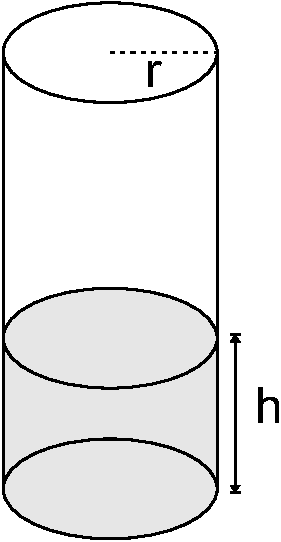
\includegraphics[height=5cm]{cylinder-rh.pdf} 
		};
		\node[inner sep=0pt,text width=0.5\linewidth] (myCaption) [below=of myImage]
		{\captionof{figure}{Cylinder with dimensions. $r$ is the radius and $h$ is the height of water in the tube.}};
	\end{tikzpicture}
	
	\section{Numerical Solution}
	
	For draining, the outflow rate (change in volume over time, ($Q=\frac{dV}{dt}$) is not constant. The outflow rate is proportional to the height of water in the tube, since the higher the water level the greater pressure at the bottom of the tube and the faster the outflow rate.
	\begin{equation}
		\frac{dV}{dt} \propto h
	\end{equation}
	
	Converting the proportionality statement to an equation requires us to introduce a constant ($k$). Also, recognizing that this will be an outflow rate means that the flow rate should be negative:
	\begin{equation}
		\label{eqn:flowRate}
		\frac{dV}{dt} = - k \cdot h
	\end{equation}
	
	As we saw when we were filling the cylinder, the change in height of water in the tube is given by the \textbf{change in height} equation:
	\begin{empheq}[box=\fbox]{equation}
		\label{eqn:dh_eqn}
		\Delta h = \frac{\Delta t}{\pi r^2} \; Q 
	\end{empheq}
	
	where $Q$ is $\frac{dV}{dt}$ so:
	\begin{equation}
		\Delta h = \frac{\Delta t}{\pi r^2} \; \frac{dV}{dt}
	\end{equation}
	
	So, let's substitute our flow rate equation (Eqn. \ref{eqn:flowRate}) for $\frac{dV}{dt}$ to get:
	\begin{empheq}[]{equation}
		\Delta h = \frac{\Delta t}{\pi r^2} \; (- k \cdot h )
	\end{empheq}

	which simplifies to:
	\begin{empheq}[]{equation}
		\Delta h = - \frac{\Delta t}{\pi r^2} \; k \cdot h
	\end{empheq}
	
	Important to note for the computer model, is that the height ($h$) used in this equation is the old height from the previous timestep so:
	\begin{empheq}[box=\fbox]{equation}
		\label{eqn:dh_drain}
		\Delta h = - \frac{\Delta t}{\pi r^2} \; k \cdot h_{old}
	\end{empheq}
	
	and we can still update the new height using:
	\begin{empheq}[box=\fbox]{equation}
		\label{eqn:hnew_eqn}
		h_{new} = h_{old} + \Delta h
	\end{empheq}
	
	so, in our code we just need to change this line and set up a few different constants.
	
	
	
	\subsection{Code: Draining}

	This program is based off the filling code, but for this example we ignore the filling by setting the inflow rate to zero (\textbf{Line 12}). We're using an initial height of 50 cm ($h_0 = 50$), and set the constant $k$ to be equal to one. 
	
	\textit{water-draining-fd.py}
	\begin{tikzpicture}[remember picture,overlay,shift={(current page.east)}]
		\node[anchor=north east,xshift=-1cm](myImage){
			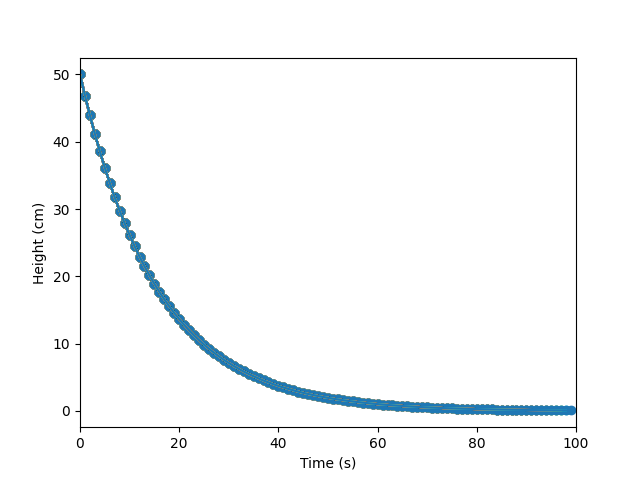
\includegraphics[height=5cm]{water-draining-fd.png} 
		};
		\node[inner sep=0pt,text width=0.5\linewidth] (myCaption) [below=of myImage]
		{\captionof{figure}{\label{drainingModel} Model output: Graph of height of water in the column over time when draining the cylinder via a hole in the bottom.  }};
	\end{tikzpicture}
	
	\lstinputlisting[language=Python, frame=single]{../water-draining-fd.py}
	
	
	The output from the model (Fig. \ref{drainingModel}) looks like an exponential decay curve, which is what we will find from the analytical solution (Eqn. \ref{analyticalDraining}).
	
	
	
	\section{Draining: Analytical Solution using Calculus}
	Experiments (which you may have done) show that if you're draining a cylinder by gravity the outflow rate of water is linearly proportional to the height of water in the tube. 
	\begin{equation}
		\frac{dV}{dt} \propto h
	\end{equation}
	
	Converting the proportionality statement to an equation requires us to introduce a constant ($k$):
	\begin{equation}
		\label{DrainingDiffEqn}
		\frac{dV}{dt} = k h
	\end{equation}
	
	So in draining, the outflow rate ($\frac{dV}{dt}$) is not constant, it slows down as the height of water in the tube decreases. 
	
	Now, lets substitute the equation for the volume of a cylinder:
	\begin{equation}
		V = \pi r^2 h
	\end{equation}
	
	into the draining equation (Eq. \ref{DrainingDiffEqn}) to get:
	\begin{equation}
		\frac{d[\pi r^2 h]}{dt} = k h
	\end{equation}
	
	we can extract $\pi$ and $r^2$ from the differential because they are constant:
	\begin{equation}
		\pi r^2 \frac{dh}{dt} = k h
	\end{equation}
	
	separating the variables gives:
	\begin{equation}
		\pi r^2 \frac{dh}{h} = k \cdot dt
	\end{equation}
	and rearranging:
	\begin{equation}
		\frac{dh}{h} = \frac{k \cdot dt}{\pi r^2 }
	\end{equation}
	\begin{equation}
		\frac{dh}{h} = \frac{k}{\pi r^2 } dt
	\end{equation}
	
	To simplify a little, lets consolidate the constants on the left hand side into one variable $K$:
	\begin{equation}
		K = \frac{k}{\pi r^2 }
	\end{equation}
	so:
	\begin{equation}
		\frac{dh}{h} = K \cdot dt 
	\end{equation}
	
	which we can integrate (remember $K$ is a constant):
	\begin{align}
		\int \frac{dh}{h} &= K \int dt \\
		\ln{h} &= K \cdot t + c
	\end{align}
	
	we can solve for $h$ by raising both sides by $e$ to cancel the $\ln$:
	\begin{equation}
		e^{\ln{h}} = e^{K t + c}
	\end{equation}
	
	\begin{equation}
		h = e^{K t + c}
	\end{equation}
	
	Because of math, we can pull the constant out to get:
	\begin{equation}
		h = Ce^{K t}
	\end{equation}
	
	Where the constant is the initial value of the height ($h_0$):
	\begin{empheq}[]{equation}
		\label{analyticalDraining}
		h = h_0 \cdot e^{K t}
	\end{empheq}
	
	This is an exponential function. If $K$ is less than 1 ($K<1$) then this is a decay curve.
	
	
\chapter{Model Calibration}
	
	We have a model that shows the general patterns we expect when filling and draining the tube: linear increase for filling at a constant rate, and exponential decay for draining due to gravity. But can these models reflect the actual thing?
	
	Fortunately, we have some experimental data, thanks to my pre-Calculus class. 
	
	We'll start with the filling portion of the model.
	
	\section{Filling Calibration}
		\begin{tikzpicture}[remember picture,overlay,shift={(current page.east)}]
			\node[anchor=north east,xshift=-1cm](myImage){
				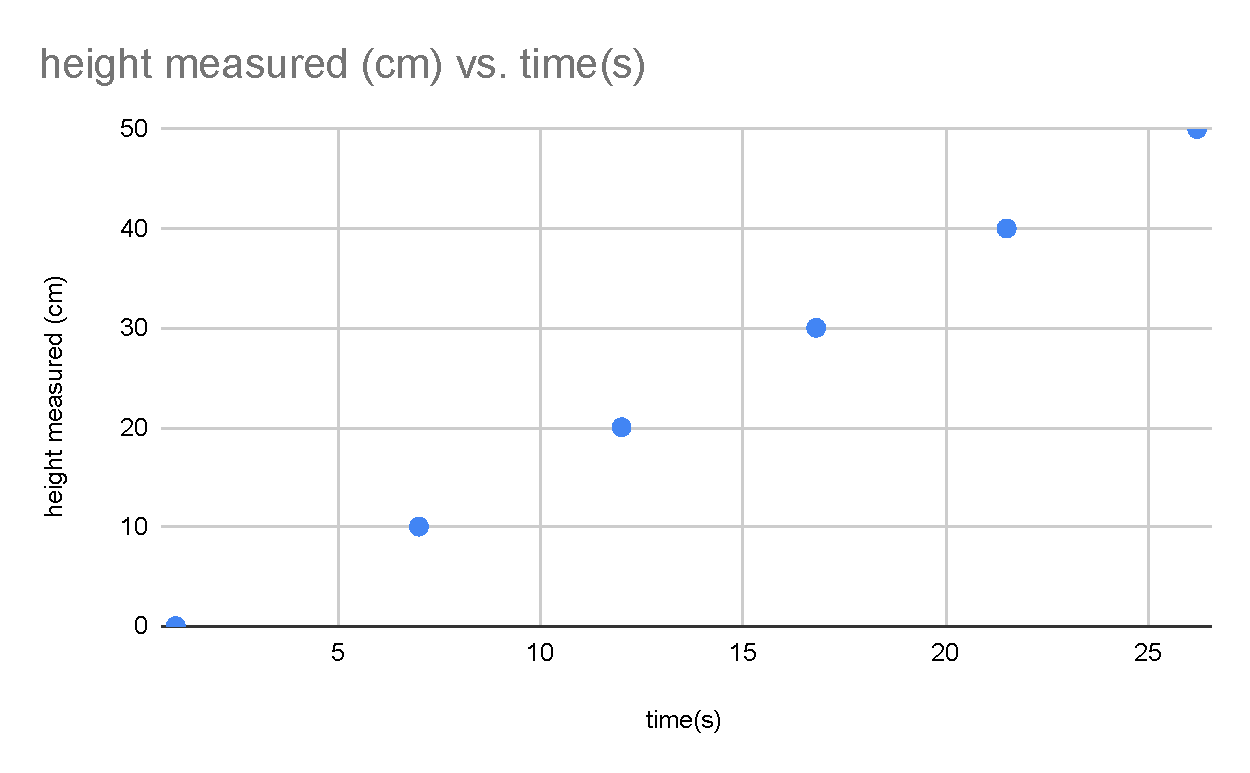
\includegraphics[width=6cm]{filling-data.pdf} 
			};
			\node[inner sep=0pt,text width=0.5\linewidth] (myCaption) [below=of myImage]
			{\captionof{figure}{\label{drainingModel} Experimental data from filling the cylinder. Data by Blas. }};
		\end{tikzpicture}	
		\begin{table}[h!]
			\centering
			\begin{tabular}{||c | c||} 
				\hline
				time (s) & height (cm) \\ [0.5ex] 
				\hline\hline
				1	& 0 \\
				7	& 10 \\
				12	& 20 \\
				16.8	& 30 \\
				21.5	& 40 \\
				26.2	& 50 \\ [1ex] 
				\hline
			\end{tabular}
			\caption{Experimental Data from filling the cylinder. Data by Blas.}
		\end{table}
	
	
	Recall that, at the core of the model, is the change in height equation (Eqn. \ref{dh_eqn}):
	\begin{empheq}[]{equation*}
		\Delta h = \frac{\Delta t}{\pi r^2} \; Q 
	\end{empheq}
		
	The radius ($r$) is measured and we choose $\Delta t$ as steps in the simulation, so the only unknown is the inflow rate ($Q$).
	
	Therefore, to calibrate the model we adjust $Q$ until the model output matches the experimental data.
	
	\begin{figure}[h!]
		\begin{center}
		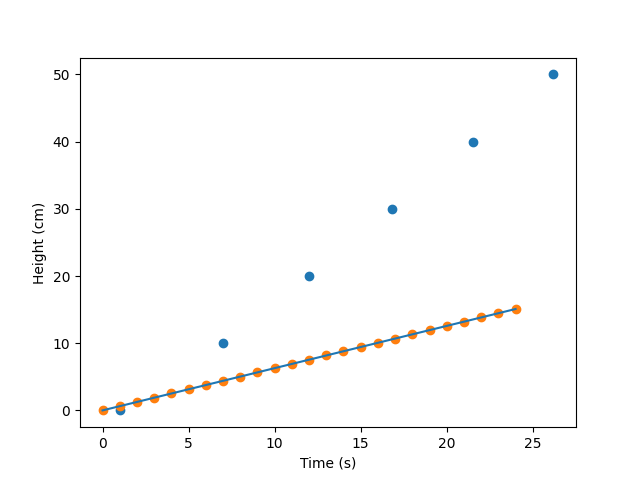
\includegraphics[width=0.75\textwidth]{filling-calibration-Q=10.png}
		\caption{Comparison of measured (blue) and modeled (red) data. This version of the model uses $Q=10$ cm$^3$/s.}
		\end{center}
	\end{figure}
	
	In order to produce this graph, we use the \textit{ezGraphMM} class, which allows us to plot the measured and modeled data separately. The full code is here:
	
	\textit{water-filling-calibration.py}
	\lstinputlisting[language=Python, frame=single]{../water-filling-calibration.py}
	
	
	\section{Calibration Analysis: r$^2$}
	
		To determine how good a match we have (instead of just eyeballing it) we'll calculate the regression coefficient ($r^2$) value using a series of assignments.
	
		\subsection{Selecting time data}
		\textbf{Assignment \qn}: 
		
		Adapt the model so it records the water heights (in an array) at the same times as the measured data (you may round the measured times to whole integers to make it easier).
		
		\subsection{Sum of the errors/residuals}
		\textbf{Assignment \qn}: 
		
		Write a function that takes the measured heights and the corresponding modeled heights and returns the \textbf{sum of all the errors} ($e$). The \textit{error} is simply the difference between the measured and the modeled value. The error is sometimes referred to as the \textbf{residual}.
		\begin{equation}
			e = h_{measured} - h_{modeled}
		\end{equation}
		so your function should return the sum of all the errors ($E$):
		\begin{equation}
			E = \sum e = \sum (h_{measured} - h_{modeled})
		\end{equation}
	
		\subsection{Differences from the mean}
		\textbf{Assignment \qn}:
		
		Write a function that finds the sum of all the differences between the measured heights and their mean ($\mu$).
		\begin{equation}
			D = \sum (h_{measured} - \mu)
		\end{equation}
	
		\subsection{$r^2$}
		\textbf{Assignment \qn}:
		
		The regression coefficient ($r^2$) is given by one minus the sum of all the errors squared divided by the sum of the differences from the mean squared:
		\begin{equation}
			r^2 = 1 - \frac{E^2}{D^2}
		\end{equation}
		Write a function that calculates the $r^2$ value.
	
	
	\section{Draining Calibration}
		\begin{tikzpicture}[remember picture,overlay,shift={(current page.east)}]
			\node[anchor=north east,xshift=-1cm](myImage){
				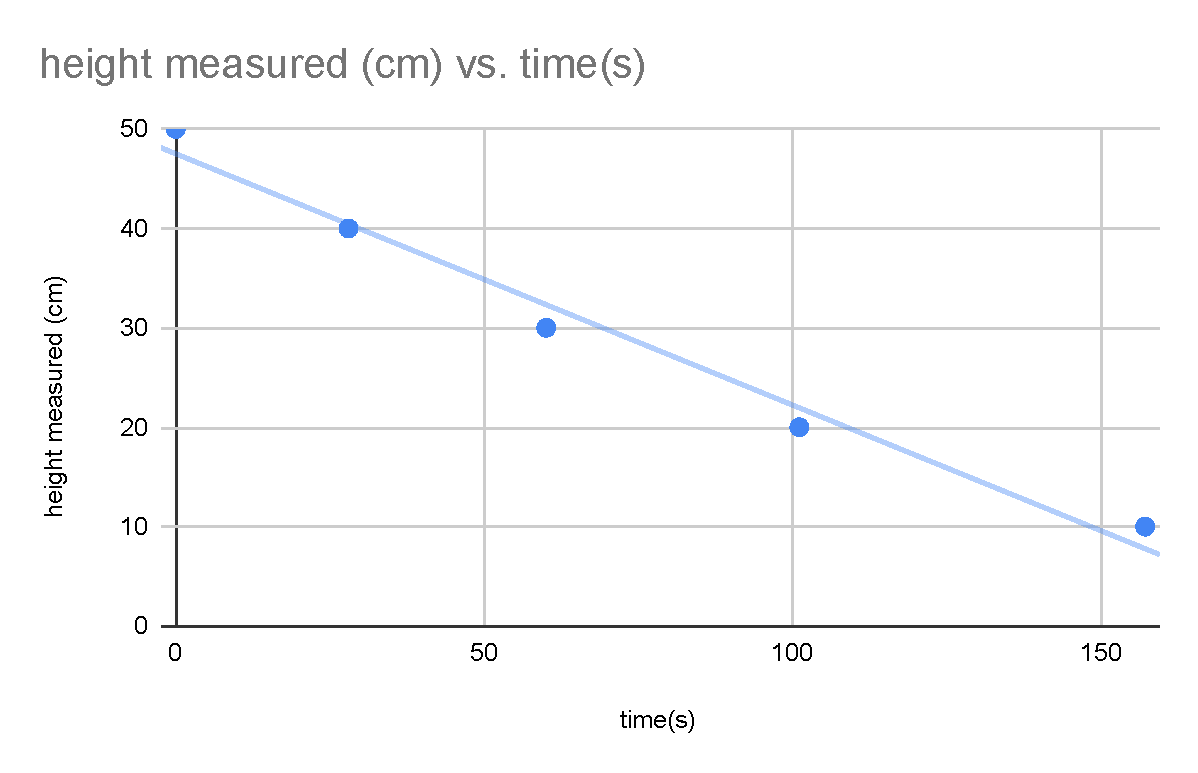
\includegraphics[width=6cm]{draining-data.pdf} 
			};
			\node[inner sep=0pt,text width=0.5\linewidth] (myCaption) [below=of myImage]
			{\captionof{figure}{\label{drainingModel} Experimental data from draining the cylinder. A linear trendline is included to highlight the curvature of the data. Data produced by Coen and Blas.}};
		\end{tikzpicture}	
		\begin{table}[h!]
			\centering
			\begin{tabular}{||c | c||} 
				\hline
				time (s) & height (cm) \\ [0.5ex] 
				\hline\hline
				0	& 50 \\
				28	& 40 \\
				60	& 30 \\
				101	& 20 \\
				157	& 10 \\ [1ex] 
				\hline
			\end{tabular}
			\caption{Experimental Data from draining the cylinder. Data by Coen and Blas.}
		\end{table}
	
	\textbf{Assignment \qn}: 
	
	Use this experimental data to calibrate the draining portion of the model.
	

	
	
	\section{Breaking the Model}
		Experiment by changing the parameters to find the limits of the model. Questions to ask are:
		
		\begin{enumerate}
			\item What is the largest timestep you can use with this model.
			\item What happens when you change the $k$ coefficient? How large can you make it?
		\end{enumerate}
	
		What you should find is that at for some values the model starts to oscillate out of control. This is one of the limitations of finite difference models. It requires pretty extreme settings in this example, but other models the unstable parameter values can be much closer to the values we want to use.
	
	
\chapter{Expanding the Model}

	As we've seen, modifying the basic model for different conditions can be pretty easy. In the base model (water filling) the change in height equation (Eqn. \ref{dh_eqn}) was:
	\begin{empheq}[]{equation*}
		\Delta h = \frac{\Delta t}{\pi r^2} \; Q 
	\end{empheq}
	
	To adjust for draining (Eqn. \ref{eqn:dh_drain}), we just needed to make the inflow value ($Q$) an equation that adjusts for the fact that the water outflow rate is negative and depends on the height of water in the tube.
	\begin{empheq}[]{equation*}
		\Delta h = \frac{\Delta t}{\pi r^2} \; (- k \cdot h)
	\end{empheq}
	
	
	
	\section{Simultaneously Filling and Draining}
		\begin{tikzpicture}[remember picture,overlay,shift={(current page.east)}]
			\node[anchor=north east,xshift=-1cm](myImage){
				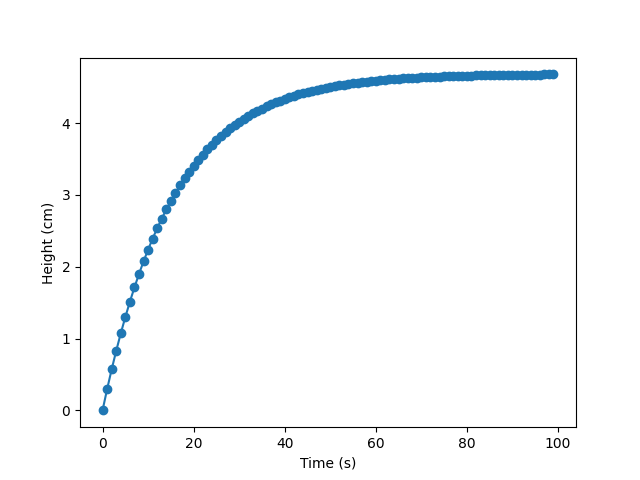
\includegraphics[height=5cm]{water-fill-and-drain.png} 
			};
			\node[inner sep=0pt,text width=0.5\linewidth] (myCaption) [below=of myImage]
			{\captionof{figure}{\label{drainingModel} The model indicates that filling the cylinder while the hole is still open would result in the water rising to an equilibrium height of about 4.7 cm. }};
		\end{tikzpicture}
		
		Our program is already set up to handle filling and draining. We simply need to change the inflow value ($Q_{in}$). 
		
		
		\textbf{What happens if we try to fill the tube while the hole in the bottom is open so it simultaneously drains?}
		
		Set the inflow value to 5 cm$^3$/s, set the initial height ($h$) to 0, and keep the draining parameters, we should see the water level increase until it reaches an equilibrium.
		
		\textbf{Model Equilibrium}: Now, if you have not already, set the inflow value and $k$ coefficient to the values you got from your calibrations and determine the equilibrium height of water in the tube. 
		
	\section{Time-variable Inputs: Changing Inflow}
	
	\subsection{Stopping Inflow}
	\tcbox[colback=blue!30, colframe=blue!30!black]{
	\textbf{Assignment \qn}: 
	
		Adapt the model so that the water input stops after 50 seconds. Use the calibrated fill rate ($Q_{in}$) for the initial inflow rate, and allow the model to drain using the calibrated $k$ coefficient.
	}
		
	\subsection{Variable Inflow}

	\textbf{Assignment \qn}: 
	
		Change the model so that the water input varies in a sinusoidal (wave) pattern with the function:
		\begin{equation}
			Q = 10 \sin{(5t)} + 11
		\end{equation}
	
		Allow the model to drain using the calibrated $k$ value.

		
	\subsection{DYO Simulation}
		\textbf{Assignment \qn}: 
		
			Design your own simulation scenario and share it with the class.
		
	
	\newpage
    \section{Water Tank Exercises}

	\subsection{Rectangular Prism}
	
	\textbf{Assignment \qn}: 
	
		Create a model for the filling of a water tank that is a rectangular prism with a width of 10 cm and a length of 5 cm.
		
		\begin{figure}[h!]
			\begin{center}
				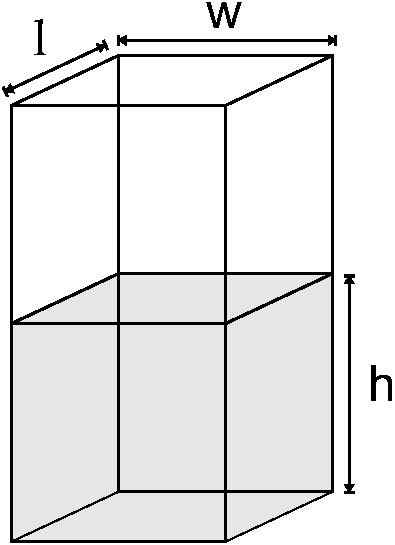
\includegraphics[height=5cm]{prism-lwh.pdf}
				\caption{Water Tank}
			\end{center}
		\end{figure}
	
	\subsection{Cone}
	\textbf{Assignment \qn}: 
	
		Create a model for the filling of a water container where the container was conical instead of a cylinder, where the radius increases by 1 cm for every 2 cm increase in height?
		
		\begin{figure}[h!]
			\begin{center}
				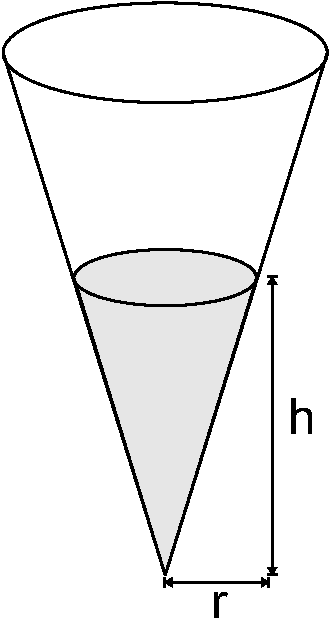
\includegraphics[height=5cm]{cone-rh.pdf}
				\caption{Conical water container.}
			\end{center}
		\end{figure}


\chapter{Ballistic Motion: A ball in the Air}

	Here we'll see how to create models based off of governing differential equations. First we attempt to find the height of a ball that is thrown upwards.
	
  \section{Acceleration and Velocity}
	For a ball flying through the air, the only force acting on it is gravity (we're ignoring friction with the air for now). If we do the physics we find that the acceleration ($a$) of a ballistic object is constant no matter the size or mass of the object.

	As we know, acceleration is the change in velocity with time so:
	\begin{empheq}[box=\fbox]{equation}
		a = \frac{dv}{dt}
	\end{empheq}

	This we can \textbf{discretize} as such:
	\begin{equation}
		\frac{dv}{dt} = \frac{\Delta v}{\Delta t}
	\end{equation}

	so that:
	\begin{equation}
	a = \frac{\Delta v}{\Delta t}
	\end{equation}

	since velocity is changing over time:
	\begin{equation}
		a = \frac{v_{new} - v_{old}}{\Delta t}
	\end{equation}

	So if we know our starting velocity ($v_{old}$) and our acceleration and set a timestep ($\Delta t$) we can solve this equation to calculate the new velocity:
	\begin{empheq}[box=\fbox]{equation}
		\label{eqn:v_new}
		v_{new} = v_{old} +  a \cdot \Delta t 
	\end{empheq}


  \section{Height and Velocity}
  	What we want to find is the height of the ball, and we do so by recalling that velocity (in an up-down direction) is the change in height ($y$) over time:
  	\begin{equation}
  		v = \frac{dy}{dt}
  	\end{equation}
  
  	Which we can discritize in the same way we did for acceleration to get a very similar equation to Eqn. \ref{eqn:v_new} to calculate height ($y$):
  	\begin{empheq}[box=\fbox]{equation}
  		\label{eqn:h_new}
  		y_{new} = y_{old} + v \cdot \Delta t
  	\end{empheq}
  	
  	With these two equations (Eqns. \ref{eqn:v_new} and \ref{eqn:h_new}), we can now create a model to simulate the height of the ball.


  \section{Model}
	
	\subsection{Parameters}
	First we set our \textbf{parameters}. Acceleration due to gravity ($g$) is:
	\begin{equation}
		g = -9.8 \; m/s^2
	\end{equation}
	It's negative because it's acting downwards.
	
	We also need to set a timestep ($\Delta t = 0.1$)and a length for the simulation, which we set as the number of steps (45 steps).

	\subsection{Initial Values}
	Next we set the initial values:
	\begin{eqnarray}
		v_0 &= 20 \; m/s \\
		y_0 &= 0  \; m
	\end{eqnarray}
	We will also need to initialize our output, which in this case is the graph.
	
	\subsection{Time Loop}
	Run through the given number of timesteps and calculate the height in each iteration.
	
	\subsection{Code}
	The final code may look like this:

	\lstinputlisting[language=Python, frame=single]{../ball.py}
	


  \section{Analysis}
  
  	\subsection{Maximum Height}
  	Assignment \qn:
  	
  	Have your program find the maximum height of the ball and the time when it reaches it. Compare your result to the analytical solutions (look them up).

	\subsection{Hitting the Ground}
	Assignment \qn:
	
	Have your program find the moment when the ball hits the ground.
	

\chapter{Energy Balance Model}

	If there were no atmosphere, what would the average temperature at the surface of the Earth?

 % Stop your text
 \end{document}
